\section{Approach}
Given a video \(X_{0:T}\) with missing regions, STSENet targets to recover the complete video \(Y_{0:T}\), where $T$ is the total number of frames.
\( \widetilde{Y}_{0:T}\) is denoted as the ground truth video, and \(M_{0:T}\) is the mask sequence that indicates the missing regions in \(X_{0:T}\).
In each inference batch, to generate current frame \(Y_t\), total $5$ frames $\boldsymbol{X}$, indexed by (\(X_{t-7}, X_{t-3}, X_{t} ,X_{t+3}, X_{t+7}\)), are fed to STSENet, as well as corresponding mask $\boldsymbol{M}$.  
%$t$ is the index of the current frame.
%The ground truth video is \( \widetilde{Y}_{0:T}\). We use \(X_t\) to denote the \(t_{th}\) input frame, while the mask \(M_{0:T}\) indicates the missing region.
%The corresponding output video frame is \(Y_t\). To generate a precise \(Y_t\), we fed the network with neighbor frames $\boldsymbol{X}$, namely, (\(X_{t-7}, X_{t-3}, X_{t} ,X_{t+3}, X_{t+7}\)) and their corresponding masks $\boldsymbol{M}$, namely, (\(M_{t-7}, M_{t-3}, M_{t} ,M_{t+3}, M_{t+7}\)), which will help the network to borrow complementary information from different frames.
The intuition is that there exists complementary information in the neighbouring frames, which can benefit the inpainting process of the current frame.
As shown in Fig.~\ref{zong}, the architecture of our network is composed of three parts: a) an edge completion module that recovers spatial details of input frames; b) a flow completion module that completes motion between neighbor frames and target frame; and c) a frame inpainting module that generates spatio-temporal consistent frames with auxiliary inpainted edge and flow.
The detailed implementation of each part will be illustrated in the following sections.



%Our network is to recover the video \(Y_{0:T}\) from the incompleted video \(X_{0:T}\). The ground truth video is \( \widetilde{Y}_{0:T}\). We use \(X_t\) to denote the \(t_{th}\) input frame, while the mask \(M_t\) indicates the missing region. The corresponding output video frame is \(Y_t\). To generate a precise target frame \(Y_t\), we fed the network with neighbor frames $\boldsymbol{X}$, namely, (\(X_{t-7}, X_{t-3}, X_{t} ,X_{t+3}, X_{t+7}\)) and their corresponding masks $\boldsymbol{M}$, namely, (\(M_{t-7}, M_{t-3}, M_{t} ,M_{t+3}, M_{t+7}\)), which will help the network to borrow complementary information from different frames. The intuition is that there may exist relative information of the unseen part in current frame in other frames, which can aid the recovery process of the target frame.
%As shown in Fig.~\ref{zong}, the architecture of our network is composed of three parts, i.e., an edge completion module, a flow completion module, and a frame inpainting module. We will introduce details of each module in the following section. 



\subsection{Edge Inpainting Network}
Video inpainting suffers from the lack of structural details.
To generate an inpainting result with fine details, we first predict corresponding reasonable structural clues, which will aid the following frame inpainting process.
%The edge completion module aims to generate the completed edge maps $\boldsymbol{E}$ for input frames $\boldsymbol{X}$. 

Given the incompleted grayscale images $\boldsymbol{X}^{g}$ of input frame, a canny edge detector is first used to generate initial edge maps $\boldsymbol{E}^{i}$. 
Then, an edge inpainting network (ENet) is designed to refine $\boldsymbol{E}^{i}$.
The input of ENet is a triplet of grayscale images, initial edge maps, and corresponding masks. 
The detailed implementation of ENet is shown in Fig.~\ref{enet}, which consists of a generator $N^E$ and a discriminator $D^E$.
$N^E$ contains a 2-layer 3D encoder, eight 2D residual blocks, and a 2-layer 3D decoder. The 3D encoder and decoder are designed to learn spatio-temporal information, while the 2D residual blocks are used to enrich the spatial features in a larger receptive field. The discriminator $D^E$ follows $70\times 70$ PatchGAN architecture \cite{Isola_2017_CVPR}.
Finally, the inpainted edge maps are obtained by:
\begin{equation}
	\label{eq:edgenet}
	\boldsymbol{E}=N^E(\boldsymbol{E}^{i},\boldsymbol{X}^{g},\boldsymbol{M}),
\end{equation}

The loss function for ENet is:
\begin{equation}
	\label{eq:loss_e}
	\mathcal{L}_{edge}=\mathcal{L}^E_{adv}+\lambda_1 * \mathcal{L}^E_{fm}
\end{equation}
where $\mathcal{L}^E_{adv}$ and $\mathcal{L}^E_{fm}$ are respectively the adversarial loss and feature matching loss. 
$\lambda_1$ is a hyper-parameter to balance different terms.
Following the adversarial learning manner, $\mathcal{L}^E_{adv}$ can facilitate ENet to produce realistic edge maps. The adversarial loss are defined by:
\begin{equation}
	\label{eq:edge_adver}
	\mathcal{L}^E_{adv}=\min\limits_{N^E} \max \limits_{D^E}\mathbb{E}[logD^E(\boldsymbol{E}^{gt},\boldsymbol{X}^{g})]+\mathbb{E}log[1-D^E(\boldsymbol{E},\boldsymbol{X}^{g})],
\end{equation}

where $E^{gt}$ represents the ground truth of edge maps 

$\mathcal{L}^E_{fm}$ evaluates the feature-level similarity between ground truth edge maps and predicted edge maps, which helps to create structurally rational edge maps. The feature matching loss is defined by:
\begin{equation}
	\label{eq:edge_fm}
	\mathcal{L}^E_{fm}=\sum_{k=1}^L{\frac{1}{N_k}\left\| D^E_k(\boldsymbol{E}^{gt},\boldsymbol{X}^{g})- D^E_k(\boldsymbol{E},\boldsymbol{X}^{g})\right\|_1},
\end{equation}
where $D^E_k$ denotes the $k$-th layer of $D^E$, while $N_k$ is the element number of the $k$-th layer.
\begin{figure}[t]
	\centering
	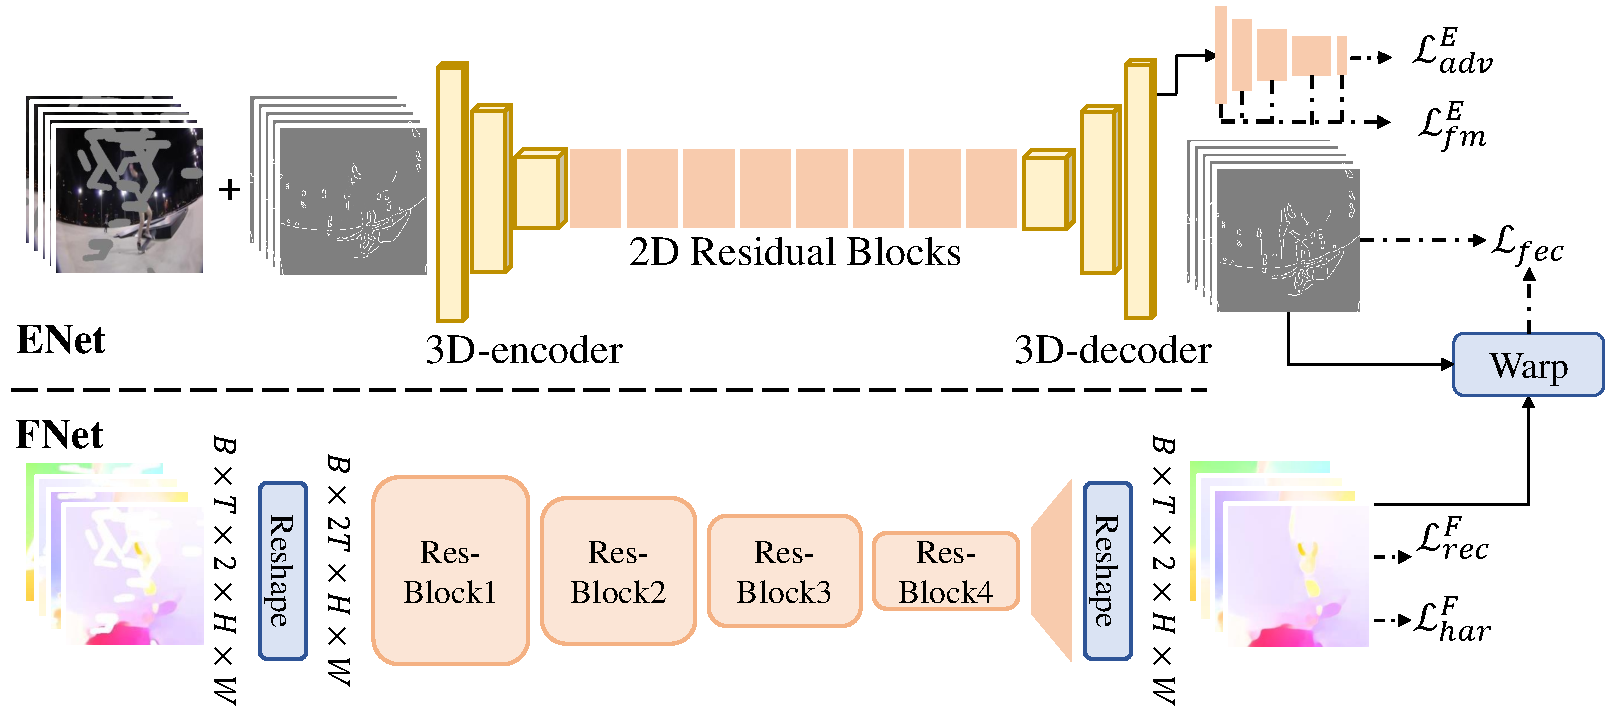
\includegraphics[width=1.1\columnwidth]{enet} % Reduce the figure size so that it is slightly narrower than the column. Don't use precise values for figure width.This setup will avoid overfull boxes. 
	\caption{The architecture of ENet and FNet. The upper is ENet, and the bottom is FNet. }
	\label{enet}
\end{figure}
\subsection{Optical Flow Completion Module}
It's important for video inpainting to maintain temporal consistency.
To this end, the optical flow completion module is designed to predict the motion tendency among frames.

Similar to ENet, the initial optical flow \(\boldsymbol{O}^i\) for $\boldsymbol{X}$ are first generated, using Flownet2.0 \cite{Flownet_2017_CVPR}.
Notably, \(\boldsymbol{O}^i\) consists of \((O^i_{t\Rightarrow t-7},O^i_{t\Rightarrow t-3},O^i_{t\Rightarrow t+3},O^i_{t\Rightarrow t+7})\).
Then, the proposed flow inpainting network (FNet) $N^F$ is used to refine \(\boldsymbol{O}^i\) by:
\begin{equation}
	\label{eq:flownet}
	\boldsymbol{O}=N^F(\boldsymbol{O}^{i},\boldsymbol{M}),
\end{equation}
where $\boldsymbol{O}$ is the refined optical flow.

The loss function for FNet is :
\begin{equation}
	\label{eq:flow_all}
	\mathcal{L}_{flow}=\mathcal{L}^F_{rec}+\mathcal{L}^F_{har},
\end{equation}
where $\mathcal{L}^F_{rec}$ and $\mathcal{L}^F_{har}$ are respectively $l_1$-reconstruction loss and hard mining loss.
The $l_1$-reconstruction loss is defined as:
\begin{equation}
	\label{eq:flow_l1}
	\mathcal{L}^F_{rec}=\frac{1}{\left\|\boldsymbol{M} \right\|_1}\left\|(\boldsymbol{O}-\boldsymbol{O}^{gt})\odot \boldsymbol{M}\right\|_1,
\end{equation}
where $\boldsymbol{O}^{gt}$ is the ground truth. The symbol $\odot$ denotes the pixel-wise multiplication. Specifically, $\mathcal{L}^F_{rec}$ measures the difference between $\boldsymbol{O}^{gt}$ and $\boldsymbol{O}$.
The hard mining loss is defined as:
\begin{equation}
	\label{eq:flow_hard}
	\mathcal{L}^F_{har}=\frac{1}{\left\|\boldsymbol{M}_H \right\|_1}\left\|(\boldsymbol{O}-\boldsymbol{O}^{gt})\odot \boldsymbol{M}_H\right\|_1,
\end{equation}
where $\boldsymbol{M}_H$ is the binary mask of hard example regions. 
The hard mining loss encourages the network to focus on those hard samples, which can avoid blurred texture. 

\subsection{Flow-Edge Consistency Loss}
Instead of separate training of ENet and FNet, we train the two networks jointly
The intuition is that the temporal information and structural details can boost each other. Thus we will obtain detail-aware optical flow and temporal consistent edge maps.

To achieve this goal, a flow-edge consistency loss is designed by:
\begin{equation}
	\label{eq:flow_edge}
	\mathcal{L}_{fec}=\sum_{k}\frac{1}{\left\|M_{t-k} \right\|_1}\left\|(E_{t}-\phi(O_{t\Rightarrow t-k},E_{t-k}))\odot M_{t-k}\right\|_1,
\end{equation}
where 
$\phi(O_{t\Rightarrow t-k},E_{t-k})$ is the flow warping operation which use optical flow $O_{t\Rightarrow t-k}$ to warp $Y_{t-k}$ and $k$ denotes the indexes of neighbor frames ($k\in \left\{-7,-3,+3,+7 \right\}$). 
$\mathcal{L}_{fec}$ warps edge maps from neighbor frames to target frame and calculates the differences between neighbor edge maps and current edge map, which forces the predicted edge maps to be consistent along time.
The output optical flow will become sharp in boundary while the edge maps will be temporal consistent.
Thus, we train the FNet with loss:
\begin{equation}
	\label{eq:flow}
	\mathcal{L}_{F}=\mathcal{L}_{flow}+\mathcal{L}_{fec}.
\end{equation}
The ENet is trained by:
\begin{equation}
	\label{eq:edge}
	\mathcal{L}_{E}=\mathcal{L}_{edge}+\mathcal{L}_{fec}.
\end{equation}






\begin{figure}[t]
	\centering
	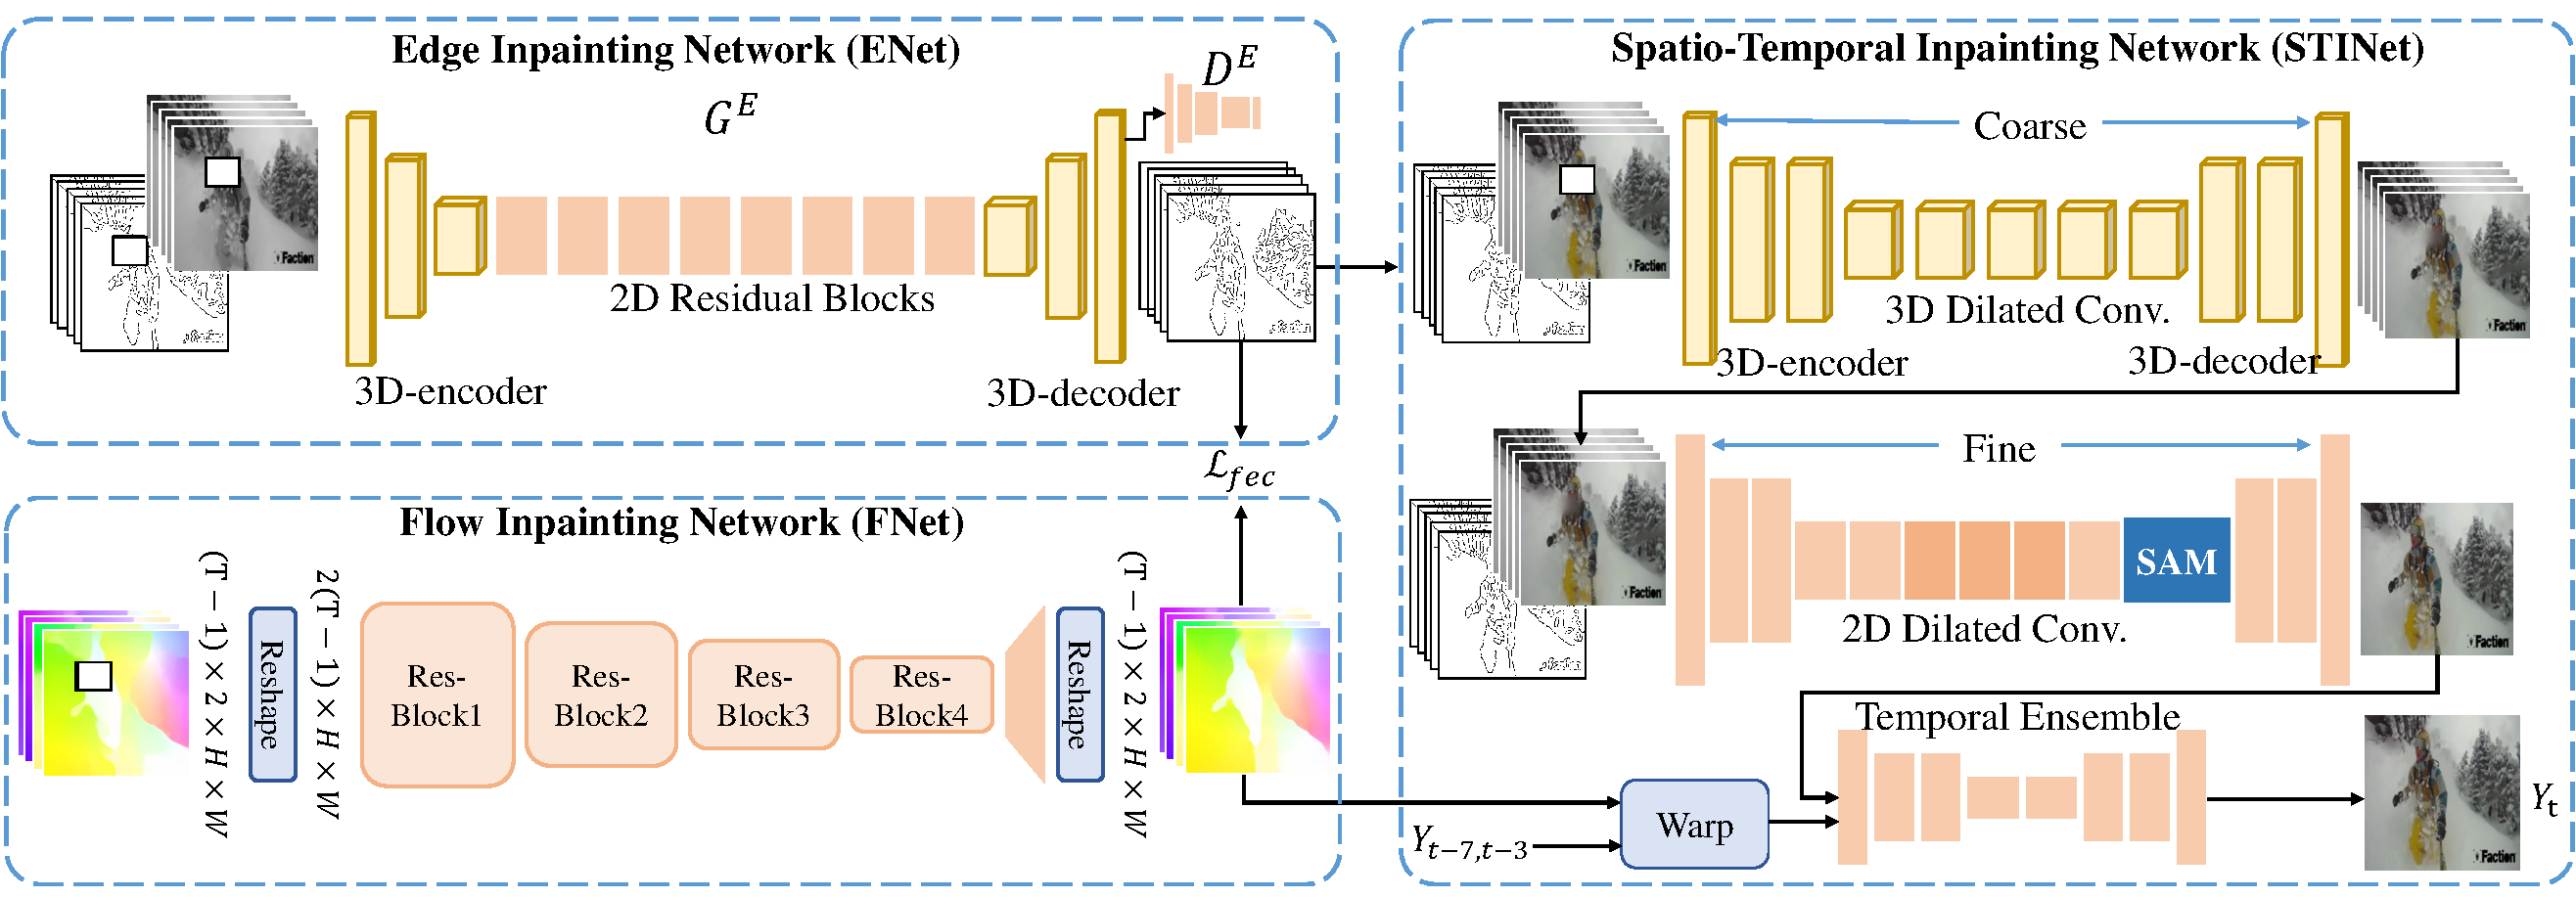
\includegraphics[width=0.95\columnwidth]{sti} % Reduce the figure size so that it is slightly narrower than the column. Don't use precise values for figure width.This setup will avoid overfull boxes. 
	\caption{The architecture of spatio-temporal inpainting (STI) module. The }
	\label{sti}
\end{figure}
\subsection{Spatio-Temporal Inpainting (STI) Module}
With both inpained edges and flow for input frames, a spatio-temporal inpainting (STI) module is designed to obtain the final target frame.
Notably, the inpained edge and flow can respectively provide structural details and temporal information.
%under the guidance of the  and motion tendency, which is helpful to the completion process of the target frame...

STI takes a combination of $\boldsymbol{X}$, $\boldsymbol{E}$ and $\boldsymbol{M}$ as input and generate the target frame $Y_t$.
As shown in Fig. \ref{sti}, STI adopts a coarse-to-fine architecture $N^I$ where the first 3D CNN network predicts an initial rough completed frame set $\boldsymbol{Y}^i$, i.e., \(Y^i_{t-7},Y^i_{t-3},Y^i_{t},Y^i_{t+3},Y^i_{t+7}\), and the second 2D CNN network refines the initial prediction to produce the final accurate output. 

To efficiently embed structure information into the network, we use the edge maps as one of the input. Besides, we propose an edge attention mechanism to force the network to focus more on the generation of hard edge regions.
The edge attention takes $\boldsymbol{E}$ as input and contains two stacked convolution layers. Then it is used as spatial attention to encourage the intermediate features of the network to attend to boundaries.
%help the intermediate feature maps  network learn details in the which 
%3D-2D CNN architecture  to model the frame inpainting with spatio-temporal consistency. 
%The input is first fed into a 3D CNN, producing an initial completed frame set . Then we use a 2D CNN to refine $\boldsymbol{Y}^i$ and generate the target $Y_t$.

With the edge-guided inpainting result, we then utilize the optical flow to smooth temporal flickers and aggregate complementary information from the neighbor frame to target frame.
Specifically, a flow warping loss is proposed:
\begin{equation}
	\label{eq:inp_flow}
	\mathcal{L}^I_{flo}=\sum_{t=1}^{T_1}\frac{1}{\left\|M^F_{t\Rightarrow t-3}\right\|_1}\left\| Y_t-\phi(O_{t\Rightarrow t-3},Y_{t-3}) \right\|_1,
\end{equation}
where $T_1$ is set to $5$ in our paper. $\phi(O_{t\Rightarrow t-3},Y_{t-3})$ is the flow warping operation which uses optical flow $O_{t\Rightarrow t-3}$ to warp the inpainted $Y_{t-3}$. $\mathcal{L}^I_{flo}$ demands few differences between warped frames and the current frame, which forces the predicted frames to be consistent through time dimension.

%\(O_{t\Rightarrow t-3}\) is used to warp the inpainted $Y_{t-3}$ to aid the current $Y_{t}$, which provides a high temporal coherence.


%, which will generate a temporal smooth fine-detailed $Y_{t}$.
The loss function for STI is:
\begin{equation}
	\label{eq:inpain_all}
	\mathcal{L}_{inp}=\mathcal{L}^{I}_{rec}+\mathcal{L}^I_{adv}+\mathcal{L}^I_{flo},
\end{equation}
where $\mathcal{L}^{I}_{rec}$, $\mathcal{L}^I_{adv}$, and $\mathcal{L}^I_{flo}$ are respectively reconstruction loss, adversarial loss and flow warping loss.
We will introduce $\mathcal{L}^{I}_{rec}$ and $\mathcal{L}^I_{adv}$.
The reconstruction loss consists of three terms:
\begin{equation}
	\begin{aligned}
		\mathcal{L}^{I}_{rec}=&\frac{1}{\left\|\boldsymbol{M} \right\|_1}\left\|(\boldsymbol{Y}^i-\widetilde{\boldsymbol{Y}})\odot \boldsymbol{M}\right\|_1 +\frac{1}{\left\|M_t \right\|_1}\left\|(Y_t-\widetilde{Y}_t)\odot M_t\right\|_1\\
		&+\mathbb{E}[\sum_{j}\frac{1}{N_j}\left\|\boldsymbol{\psi}_j(\widetilde{Y}_t)-\boldsymbol{\psi}_j(Y_t)\right\|_1]\\
		&+\mathbb{E}_j[\left\|G^{\boldsymbol{\psi}_j}(\widetilde{Y}_t)-G^{\boldsymbol{\psi}_j}(Y_t)\right\|_1],
	\end{aligned}
\end{equation}
where the first line is pixel l1 loss. The second line is the perceptual loss \cite{gatys2015neural}, which is to compare contents of the generated frame and ground truth frame.
$\boldsymbol{\psi}_j$ denotes the activation maps of $j_{th}$ layer in a network.
$N_j$ is the number of elements in layer $\boldsymbol{\psi}_j$. We use layers $relu_{1\_1}$, $relu_{2\_1}$, $relu_{3\_1}$, $relu_{4\_1}$ and $relu_{5\_1}$ of the VGG-19 network pre-trained on the ImageNet dataset for this loss. The third line is the style loss, designed to prevent "checkerboard" artifacts \cite{Sajjadi_2017_ICCV} caused by transpose convolution. $G^{\boldsymbol{\psi}_j}$ is the Gram matrix calculated by auto-correlation of $\boldsymbol{\psi}_j$. The layers are the same as that of perceptual loss.

%The adversarial loss is only for the final $Y_{t}$
The adversarial loss are defined as:
\begin{equation}
	\label{eq:inp_adver}
	\mathcal{L}^I_{adv}=\min\limits_{N^I} \max \limits_{D^I} \mathbb{E}[logD^I(\widetilde{Y}_t)]+\mathbb{E}log[1-D^I(Y_{t})],
\end{equation}
where $D^I$ possesses the same architecture as that of $D^E$, except the input dimension.

%The flow warping loss is to strengthen temporal smoothness and alleviate flickers, which is defined as:

















%Edge-preserved inpainting brunch is to recover a fine-detailed inpainting results, which is presented in blue in Fig.~\ref{zong}. This brunch is composed of three stages, canny edge detector, edge inpainting network and edge-guided inpainting network.
%To recover the \(t_{th}\) frame \(Y_t\), we adopt a multi-to-single frame inpainting strategy.  To obtain more complementary information, we fed the brunch with five frames, namely, \(X_{t-7},X_{t-3},X_{t},X_{t+3},X_{t+7}\).

%The first stage takes grayscale images of the five frames as input and uses canny edge detector to  